\chapter{Aufbau}
Im Folgenden wird der Aufbau der Simulation zunächst theoretisch und abstrahiert betrachtet. 
Folgende Notation soll jedoch eine Verknüpfung mit dem Quellcode vereinfachen: \code{Name im Quellcode}
\begin{figure}
    \centering
    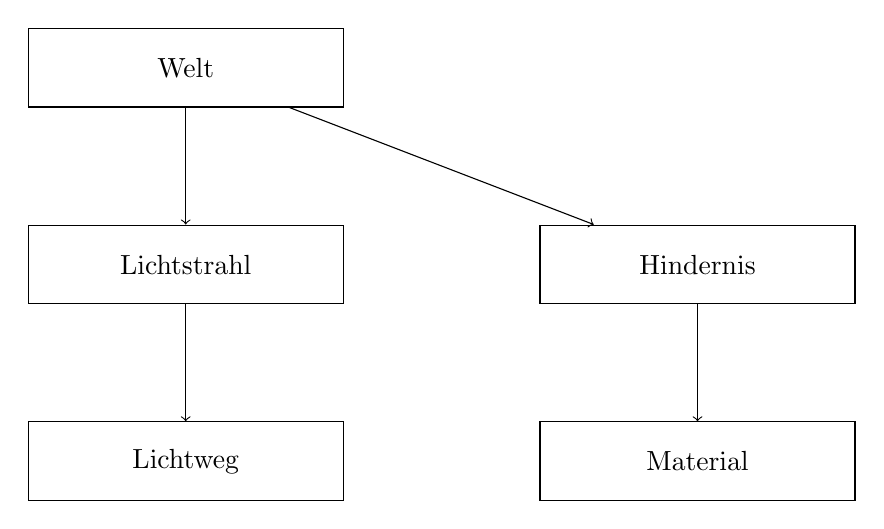
\begin{tikzpicture}[node distance=2.5cm, every node/.style={fill=white, draw=black}, align=center, minimum width=4cm, minimum height=1cm, text centered]
        \node(world)[rectangle]{Welt};
        \node(ray)[rectangle, below of=world]{Lichtstrahl};
        \node(line)[rectangle, below of=ray]{Lichtweg};
        \node(obstacle)[rectangle, right of=ray, xshift=4cm]{Hindernis};
        \node(material)[rectangle, below of=obstacle]{Material};

        \draw[->] (world) -- (ray);
        \draw[->] (world) -- (obstacle);
        \draw[->] (ray) -- (line);
        \draw[->] (obstacle) -- (material);
    \end{tikzpicture}
    \caption{Schematischer Aufbau der Simulation \\ Quelle: Eigene Darstellung}
    \label{m1}
\end{figure}

\section{Welt}
Die Welt \code{World} ist der Grundstein für die Simulation. 
Zu diesem virtuellen zweidimensionalen Raum können sämtliche Entitäten hinzugefügt werden. 
Hier werden diese verwaltet, verarbeitet und zur Visualisierung ausgegeben. 

\section{Lichtstrahl}
In der geometrischen Optik geht man bei einem Lichtstrahl \code{Ray} 
von einem Strahl aus, der sich von einem Ursprung $ A $  
geradlinig in eine Richtung mit dem Winkel 
$ \alpha $ ausbreitet. \parencite[vgl.][S. 1041]{tipler2015physik} mathematisch 
wird dieser als Halbgerade angesehen $ \overrightarrow{AB} $. 
In der Simulation ist es sinnvoll lediglich den Startpunkt als Ortsvektor $ \vec{O} $ \code{origin} innerhalb der Welt
und den Winkel \code{angle}, in den der Strahl ausgeht direkt zu speichern. 

\section{Lichtweg}
Es muss davon ausgegangen werden, dass ein Lichtstrahl in der 
die Kollision mit anderen Objekten seine Richtung verändert. 
Ab einer Richtungsänderung wird der bisherige Lichtstrahl als Lichtweg \code{Line} 
gespeichert, um in später zu visualisieren.
Hierbei besteht ein Lichtstrahl aus den Ortsvektoren $ \vec{O} $ \code{origin} dem 
Ursprung des Lichtstrahls und $ \vec{E} $ \code{end} dem Punkt der Kollision.

\section{Hindernis}
Bei allen Entitäten in der Welt, die nicht Strahl oder Lichtweg sind, 
handelt es sich um Hindernisse. 
Dieser definieren sich durch ihre geometrische Form und Position in der Welt 
und können von Lichtstrahlen getroffen werden.
Es sind verschiedene Variationen möglich. Jedes Hindernis \code{Obstacle} 
hat jedoch einen Startpunkt als Ortsvektor $ \vec{A} $ \code{start} in der Welt. 
Und ein Material \code{material} (vgl. \ref{material}). 
Folgende Typen wurden für diese Arbeit ausgewählt, eine Erweiterung ist jedoch möglich: 

\subsection{Kreis}
Der Kreis \code{type: 'cirlce'} hat eine zusätzliche Angabe über den Radius $ r $ \code{radius}.

\subsection{Linie}
Neben einen Anfangspunkt hat die Linie \code{type: 'line'} auch einen Ortsvektor $ \vec{B} $ als Endpunkt. 

\subsection{Kurve}
Zusätzlich kann ein Hindernis auch eine Kurve \code{type: 'curve'} sein. 
Das ermöglicht die Konstruktion verschiedener besonderer Reflektoren (z. B. Parabolischer Reflektor).
Für den Verlauf der Kurve besitzt dieser Hindernis-Typ eine Funktion $ f $. 
Um eine Kurve beliebig in der Welt zu positionieren, kann ihr zusätzlich eine Winkel $ \gamma $ \code{rotation} übergeben werden, 
der alle Punkte auf Kurve relative zum Ursprung rotiert. \\
Im Umfang dieser Arbeit wird bewusst auf eine vollständige und genaue Darstellung eines Graphen verzichtet. 
Daher werden nur Punkte in einem Interval $ [-40, 40] $ im Abstand von einer übergebene Skalierung $ k $ \code{scale} errechnet, 
als Linien verbunden und als diese Fortlaufend verarbeitet. 
Diese Annäherung ist ausreichend, während gleichzeitig der Umfang stark reduziert wird.


\section{Material}
\label{material}
Die Existenz eines Materials \code{Material} in der Welt besteht nur in der Verknüpfung zu einem Hindernis. 
Ein Material ist für die Verarbeitung eines einfallenden, mit dem Hindernis kollidierenden, Lichtstrahls verantwortlich 
und kann eine beliebig Anzahl an neuen Lichtstrahlen zurückgeben. \\ 
In dieser Arbeit wird nur die Reflexion bei dem Material Spiegel \code{mirror} behandelt. 
Eine Trennung von Material und Hindernis ermöglicht jedoch eine einfache Erweiterung.
Dabei können trotz Veränderung der strahlenoptischer Funktion, die geometrischen Eigenschaften beibehalten werden.
So könnte beispielsweise ein Kreis einerseits als Spiegel die Lichtstrahlen reflektieren 
und anderseits als Glas die Lichtstrahlen brechen. Ohne das dafür die Veränderung des Hindernisses von Nöten wäre.


\chapter{Technische Voraussetzungen}
Um die Zugänglichkeit der Simulation zu erhöhen, wird diese als Web-App programmiert. 
Dazu wird die Programmiersprache TypeScript benutzt und die Applikation wird mit dem Framework „SvelteKit“\footnote{https://kit.svelte.dev} kompiliert.
Zur Visualisierung wird die Library „Pts“\footnote{https://ptsjs.org} verwendet. Diese ermöglicht eine einfache Verwendung der Canvas-API. 
Zusätzlich werden aber auch einige mathematisch Hilfsfunktionen von dieser Library verwendet.

Der gesamte Quellcode für die Simulation ist auf GitHub aufzufinden\footnote{https://github.com/b3ngg/ray-optics-simulation}. 
Im Folgenden werden nur kleine, unvollständige Ausschnitte aus dem Code eingebunden.


\chapter{Simulationsprozess}
Im Folgenden wird nun der Ablauf der Simulation vom erstellen der Szene bis hin zum Visualisieren des Resultats beschrieben.

\section{Erstellen der Welt}
Zunächst muss für die Simulation eine Umgebung errichtet werden. Dazu wird eine Welt erstellt.
Zu dieser werden in dieser Szene ein von links oben (man beachte, dass das Koordinatensystem den 
Ursprung links oben hat und die y-Achse umgekehrt zum normalen Koordinatensystem ist) beginnender und diagonal nach rechts 
unten strahlender Lichtstrahl hinzugefügt. \\
Zudem wird auch ein Hindernis in der Form einer vertikalen Linie in der Mitte der Szene hinzugefügt. 
Diese hat das Material Spiegel \code{mirror}. \\ 
Nun wird mit \texttt{world.update()} die Simulation aktualisiert und die Lichtwege berechnet. Dieser werden zum Schluss visualisiert.

Bei den Objekt \texttt{space} handelt es sich um ein von Pts bereitgestellte und zur Visualisierung benötigte Objekt. 
Die Klasse \texttt{Pt} ist ebenfalls Teil von Pts und wird zur Vektormathematik verwendet.
\newpage

\begin{verbnobox}[\scriptsize\mbox{}]
/**
 * Simple reflection of a ray on a vertical line
 */
export const lineReflection: Scene = (space) => {
    const form = space.getForm();
    const world = createWorld();

    world.addSource('ray', createRay(new Pt(), Math.PI * 2.25));
    world.addObstacle(
        'line',
        createLine(new Pt(800, 0), { end: new Pt(800, 5000), material: mirror })
    );

    world.update();
    space.add(() => {
        world.draw(form);
    });

    space.playOnce();
};
\end{verbnobox}